\documentclass{article}
\usepackage[left=3cm,right=3cm,
    top=2cm,bottom=2cm,bindingoffset=0cm]{geometry}
\usepackage{graphicx} % Required for inserting images

\usepackage[english, russian]{babel}
\usepackage[T2A]{fontenc}			% кодировка
\usepackage[utf8]{inputenc}			% кодировка исходного текста
\usepackage{amsmath,amsfonts,amssymb,amsthm,mathtools}

\title{\textbf{Лабораторная работа 1.2.5.} \linebreak
ИССЛЕДОВАНИЕ ВЫНУЖДЕННОЙ РЕГУЛЯРНОЙ ПРЕЦЕССИИ ГИРОСКОПА}
\author{Попова Софья Б04-401}
\date{October 2024}

\begin{document}

\maketitle

\section*{Цель работы}
Исследовать вынужденную прецессию гироскопа. Установить зависимость скорости вынужденной прецессии от величины момента силы, действующей на ось гироскопа, и сравнить ее со скоростью, рассчитанной по скорости прецессии.

\section*{Оборудование}
Гироскоп в кардановом подвесе, набор грузов разной массы, секундомер, линейка с транспортиром, осциллограф.

\section*{Теоретическая часть}

\subsection*{Измерение частоты вращения ротора}
Гироскоп - быстро вращающееся твердое тело, для которого момент импульса относительно одной оси значительно больше момента импульса относительно других осей. Гироскоп уравновешен если его центр масс неподвижен.

\

\noindent
Устойчивость вращения гироскопа связана с тем, что приращение момента импульса при действии внешних сил в течение короткого промежутка времени много меньше самого момента импульса и практически не изменяет его.

\

\noindent
Рассмотрим гироскоп, вращающийся относительно оси $OZ$ со скоростью $\omega$. Для того чтобы гироскоп начал совершать регулярную прецессию вокруг оси $OY$ с угловой скоростью $\Omega$ необходимо приложить к нему момент внешних сил $\bar{M}$, направленный вдоль оси $OX$. При этом, если выполнено условие $\bar{L_{\Omega}} \ll \bar{L_{\omega}}$, то момент импульса гироскопа относительно главной оси $\bar{L}$ практически не меняется со временем по модулю и связан с моментом приложенных сил $\bar{M}$ и скоростью прецессии $\Omega$ следующим соотношением:
\begin{equation}
    \bar{M} = \frac{d\cdot\bar{L}}{d\cdot t} = \bar{\Omega}\cdot\bar{L}
\end{equation}

\noindent
Для изучения регулярной прецессии уравновешенного гироскопа подвесим к нему дополнительные грузы. Это смещает общий центр масс и создает момент силы тяжести, вызывающий прецессию. Тогда скорость вращения ротора гироскопа равна:
\begin{equation}
    \omega = \frac{L}{I_{z}} = \frac{M}{I_{z}\cdot\Omega} 
\end{equation}

\noindent
где $M = mgl$

\subsection*{Измерение момента инерции ротора}
Момент инерции ротора измеряем по периоду крутильных колебаний на жесткой проволоке. Чтобы исключить модуль кручения проволоки $f$, подвешиваем цилиндр правильной формы с известным моментом инерции $I$
\begin{equation}
     T=2\pi\sqrt{\frac{I}{f}}, \ \ \ \ \ I=I_\text{ц}\frac{T^2}{T^2_\text{ц}}
\end{equation}

\subsection*{Измерение момента сил трения}
Так как силы трения имеют составляющую, не лежащую в плоскости осей вращения, они меняют момент импульса и по направлению, и по величине. Для ротора гироскопа действие сил трения скомпенсированно электромотором, для карданова подвеса компенсации нет. В результате чего ось гироскопа будет опускаться в направлении действия груза. Момент сил трения $M_\text{тр}$ может быть вычислен по формуле: 
\begin{equation}
     M_\text{тр} = \frac{\Delta \alpha}{t}L
\end{equation}

\section*{Экспериментальная часть}
\subsection*{Измерение периода прецессии}
Для измерения периода прецессии гироскопа даем ротору гироскопа раскрутиться и подвещиваем различные по массе грузы на рычаг, укрепленный на оси гироскопа. Полученные данные представлены в таблице:

\begin{table}[h]
    \centering
    \begin{tabular}{|c|c|c|c|c|c|c|c|c|}
        \hline
              & m, г & \multicolumn{5}{|c|}{77} & $\Omega$, рад/с\\
        \cline{2-8}
            1 &       t, с      & 263,98 & 263,25 & 263,68 & 264,68 & 264,65 & \\
              &    n, обороты   &    2   &    2   &    2   &    2   &    2   & \raisebox{1.5ex}[0cm][0cm]{0,047}\\
        \hline
              & m, г & \multicolumn{5}{|c|}{174} & $\Omega$, рад/с\\
        \cline{2-8}
            2 &       t, с      & 231,56 & 232,11 & 232,77 & 233,75 & 232,50 & \\
              &    n, обороты   &    4   &    4   &    4   &    4   &    4   & \raisebox{1.5ex}[0cm][0cm]{0,11}\\
        \hline
              & m, г & \multicolumn{5}{|c|}{218} & $\Omega$, рад/с\\
        \cline{2-8}
            3 &       t, с      & 139,87 & 139,80 & 139,63 & 139,30 & 138,69 & \\
              &    n, обороты   &    3   &    3   &    3   &    3   &    3   & \raisebox{1.5ex}[0cm][0cm]{0,135}\\
        \hline
              & m, г & \multicolumn{5}{|c|}{271} & $\Omega$, рад/с\\
        \cline{2-8}
            4 &       t, с      & 149,43 & 149,53 & 149,18 & 149,21 & 148,34 & \\
              &    n, обороты   &    4   &    4   &    4   &    4   &    4   & \raisebox{1.5ex}[0cm][0cm]{0,168}\\
        \hline
              & m, г & \multicolumn{5}{|c|}{329} & $\Omega$, рад/с\\
        \cline{2-8}
            5 &       t, с      & 184,26 & 153,12 & 152,28 & 153,76 & 152,47 & \\
              &    n, обороты   &    6   &    5   &    5   &    5   &    5   & \raisebox{1.5ex}[0cm][0cm]{0,204}\\
        \hline
    \end{tabular}
\end{table}

\noindent
Для вычисления $\Omega$ используется формула $\Omega = \frac{2\pi n\pm \Delta\varphi}{t}$, где $n$ - количество оборотов, $\Delta\varphi$ - угол, на который опустилась ось ($20^\circ \approx 0,349$ рад), $t$ - время оборотов.

\

$M = mgl = m[\text{кг}]\cdot9,815[\text{м/с*с}]\cdot0,12[\text{м}] = m \cdot 0,0011778$

\

$\frac{\sigma_M}{M} = \sqrt{(\frac{\sigma_m}{m})^2 + (\frac{\sigma_l}{l})^2}$

\

$\sigma_M = M\cdot\sqrt{(\frac{0,001}{\text{от 0,077 до 0,329}})^2 + (\frac{0,001}{0,12})^2} \approx M \cdot 0,01$ - относительная погрешность $\approx 1\%$

\

$\frac{\sigma_{\Omega}}{\Omega} = \sqrt{(\frac{\sigma_t}{t})^2 + (\frac{\sigma_{\Delta\varphi}}{\Delta\varphi})^2}$

\

$\sigma_{\Omega} = \Omega \cdot \sqrt{(\frac{0,5}{\text{от 138,69 до 264,68}})^2 + (\frac{0,05}{0,349})^2} \approx \Omega \cdot 0,14$ - относительная погрешность $\approx 14\%$

\

\noindent
Зависимость $\Omega$ от $M$ представлена в графике:

\begin{figure}[h]
    \centering
    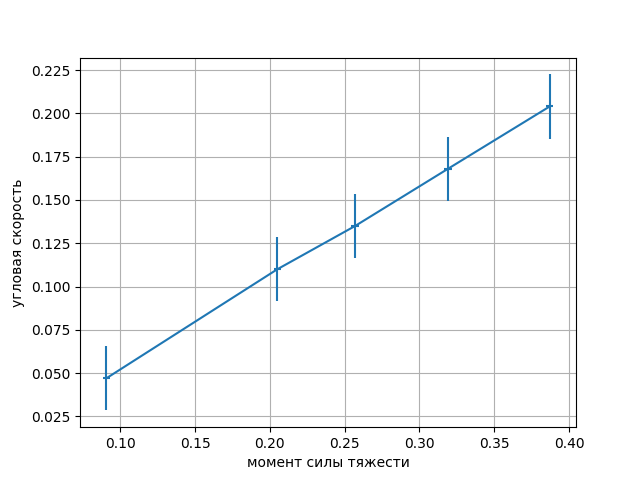
\includegraphics[width=0.75\linewidth]{Figure_1.png}
    \caption{График $\Omega$ (угловая скорость регулярной прецессии) в зависимости от $M$ (момент силы тяжести)}
\end{figure}

\

\subsection*{Измерение момента инерции}
Для измерения момента инерции ротора гироскопа относительно оси симметрии $I_0$ его подвесили к концу вертикально висящей проволоки так, чтобы ось ротора была вертикальна и измерили период крутильных колебаний получившегося маятника. После, ротор заменили цилиндром и определили период крутильных колебаний для него. 

\noindent
Полученные данные представлены в таблице:

\begin{table}[h]
    \centering
    \begin{tabular}{|c|c|c|c|}
        \hline
         & $n$ & $t$, c & $T$, с \\
         \hline
               &    & 61 & 3,05 \\
         Ротор & 20 & 63 & 3,15 \\
               &    & 64 & 3,2  \\
         \hline
                 &    & 79 & 3,95 \\
         Цилиндр & 20 & 79 & 3,95 \\
                 &    & 80 & 4    \\
         \hline
    \end{tabular}
\end{table}
$n$ - количество колебаний, $t$ - время колебаний, $T$ - период колебаний

\

\noindent
Эталонный цилиндр
\begin{itemize}
    \item Масса: 1616,3г
    \item Диаметр (5 измерений): 7,80см, 7,77см, 7,83см, 7,81см, 7,80см
\end{itemize}

\noindent
Период крутильных колебаний цилинда вычисляется по формуле: $I = \frac{m\cdot r^2}{2}$

\

\noindent
Примем период колебаний цилиндра за среднее из трех измерений, т.е. $T_\text{ц} = 3,96$с ($T = 3,13$c). Диаметр цилиндра - за среднее из пяти измерениий, т.е. $d = 7,802$см, т.е. $r = 3,901$см $= 0,03901$м $\approx 0,04$м

\noindent
Тогда $I_{\text{ц}} \approx 1,3 \cdot 10^{-3}$. По формуле (3): $I = 1,3 \cdot 10^{-3} \cdot \frac{3,13^2}{3,96^2} = 0,812 \cdot 10^{-3}$.

\

$I=\frac{m\cdot r^2}{2}\cdot\frac{T^2}{T^2_c}$ $\Rightarrow$ $\frac{\sigma_I}{I} = \sqrt{(\frac{\sigma_m}{m})^2 +(\frac{\sigma_r}{r})^2 +(\frac{\sigma_{T_\text{ц}}}{T_\text{ц}})^2 +(\frac{\sigma_T}{T})^2}$

$\sigma_I = I \cdot \sqrt{(\frac{0,05}{1616,3})^2 +(\frac{0,0005}{0,04})^2 +(\frac{0,0245}{3,96})^2 +(\frac{0,0625}{3,13})^2} \approx 0,024 \cdot I$ - отн. погрешность $\approx 2,4\%$

(Для определения $\sigma_T , \sigma_{T\text{ц}}$ используется формула $\sigma_{\text{отд}} = \sqrt{\frac{1}{n-1}\Sigma(x_i-x_{cp})^2}$ \ )

\ 

\noindent
По формуле (2) определим угловую скорость вращения ротора гироскопа: $$\omega = \frac{mgl}{I\cdot\Omega} \approx \frac{9,815 \cdot 0,12}{0,62\cdot 0,812\cdot10^{-3}} \approx 2339,5c^{-1}$$

$$\sigma_{\omega} = \omega\cdot\sqrt{(\frac{\sigma_M}{M})^2  + (\frac{\sigma_I}{I})^2+ (\frac{\sigma_\Omega}{\Omega})^2}
= \omega\cdot\sqrt{0,01 + 0,024 + 0,14} \approx 0,42\omega$$

\noindent
Используя полученную угловую скорость можно определить частоту вращения ротора гироскопа: $$v = \frac{\omega}{2\pi} \approx 372,34 \text{Гц}$$

\

\noindent
С помощью осциллографа получено значение частоты вращения ротора 378Гц

\section*{Вывод}
Значения частоты вращения ротора, полученные разными методами отличаются на 5,66Гц, что составляет погрешность 1,5\% 


\end{document}